         \chapter{Average gradient}
    \setcounter{figure}{1}
    \setcounter{subfigure}{1}
    \label{3b3f311aa3ebba82678f2a2244617492}
         \section{ Introduction and Straight-line functions}
    \nopagebreak
            \label{m39213} $ \hspace{-5pt}\begin{array}{cccccccccccc}   \end{array} $ \hspace{2 pt}\raisebox{-5 pt}{
\includegraphics[width=0.5cm]{col11306.imgs/summary_www.png}} {(section shortcode: MG10081 )} \par 
    \label{m39213*cid2}
            \subsection{ Introduction}
            \nopagebreak
      \label{m39213*id189263}The gradient of a straight line graph is calculated as:\par 
      \label{m39213*uid1}\nopagebreak\noindent{}
        \settowidth{\mymathboxwidth}{\begin{equation}
    \frac{{y}_{2}-{y}_{1}}{{x}_{2}-{x}_{1}}\tag{10.1}
      \end{equation}
    }
    \typeout{Columnwidth = \the\columnwidth}\typeout{math as usual width = \the\mymathboxwidth}
    \ifthenelse{\lengthtest{\mymathboxwidth < \columnwidth}}{% if the math fits, do it again, for real
    \begin{equation}
    \frac{{y}_{2}-{y}_{1}}{{x}_{2}-{x}_{1}}\tag{10.1}
      \end{equation}
    }{% else, if it doesn't fit
    \setlength{\mymathboxwidth}{\columnwidth}
      \addtolength{\mymathboxwidth}{-48pt}
    \par\vspace{12pt}\noindent\begin{minipage}{\columnwidth}
    \parbox[t]{\mymathboxwidth}{\large$
    \frac{{y}_{2}-{y}_{1}}{{x}_{2}-{x}_{1}}$}\hfill
    \parbox[t]{48pt}{\raggedleft 
    (10.1)}
    \end{minipage}\vspace{12pt}\par
    }% end of conditional for this bit of math
    \typeout{math as usual width = \the\mymathboxwidth}
      \label{m39213*id189656}for two points $\left({x}_{1},{y}_{1}\right)$ and $\left({x}_{2},{y}_{2}\right)$ on the graph.\par 
      \label{m39213*id189717}We can now define the \textsl{average gradient} between two points even if they are defined by a function which is not a straight line, $\left({x}_{1},{y}_{1}\right)$ and $\left({x}_{2},{y}_{2}\right)$ as:\par 
      \label{m39213*uid2}\nopagebreak\noindent{}\settowidth{\mymathboxwidth}{\begin{equation}
    \frac{{y}_{2}-{y}_{1}}{{x}_{2}-{x}_{1}}\tag{10.2}
      \end{equation}
    }
    \typeout{Columnwidth = \the\columnwidth}\typeout{math as usual width = \the\mymathboxwidth}
    \ifthenelse{\lengthtest{\mymathboxwidth < \columnwidth}}{% if the math fits, do it again, for real
    \begin{equation}
    \frac{{y}_{2}-{y}_{1}}{{x}_{2}-{x}_{1}}\tag{10.2}
      \end{equation}
    }{% else, if it doesn't fit
    \setlength{\mymathboxwidth}{\columnwidth}
      \addtolength{\mymathboxwidth}{-48pt}
    \par\vspace{12pt}\noindent\begin{minipage}{\columnwidth}
    \parbox[t]{\mymathboxwidth}{\large$
    \frac{{y}_{2}-{y}_{1}}{{x}_{2}-{x}_{1}}$}\hfill
    \parbox[t]{48pt}{\raggedleft 
    (10.2)}
    \end{minipage}\vspace{12pt}\par
    }% end of conditional for this bit of math
    \typeout{math as usual width = \the\mymathboxwidth}
      \label{m39213*id189835}This is the same as (10.1).\par 
    \label{m39213*cid3}
            \subsection{ Straight-Line Functions}
            \nopagebreak
\label{m39213*secfhsst!!!underscore!!!id141}
            \subsubsection{  Investigation : Average Gradient - Straight Line Function }
            \nopagebreak
      \label{m39213*id189861}Fill in the table by calculating the average gradient over the indicated
intervals for the function $f\left(x\right)=2x-2$. Note that (${x}_{1}$;${y}_{1}$) is the co-ordinates of the first point and (${x}_{2}$;${y}_{2}$) is the co-ordinates of the second point. So for AB, (${x}_{1}$;${y}_{1}$) is the co-ordinates of point A and (${x}_{2}$;${y}_{2}$) is the co-ordinates of point B.\par 
      \label{m39213*id189893}
    % \textbf{m39213*id189899}\par
          \begin{table}[H]
    % \begin{table}[H]
    % \\ '' '0'
        \begin{center}
      \label{m39213*id189899}
    \noindent
    \tabletail{%
        \hline
        \multicolumn{6}{|p{\mytableboxwidth}|}{\raggedleft \small \sl continued on next page}\\
        \hline
      }
      \tablelasttail{}
      \begin{xtabular}[t]{|l|l|l|l|l|l|}\hline
         &
                  ${x}_{1}$
                 &
                  ${x}_{2}$
                 &
                  ${y}_{1}$
                 &
                  ${y}_{2}$
                 &
                  $\frac{{y}_{2}-{y}_{1}}{{x}_{2}-{x}_{1}}$
                % make-rowspan-placeholders
     \tabularnewline\cline{1-1}\cline{2-2}\cline{3-3}\cline{4-4}\cline{5-5}\cline{6-6}
      %--------------------------------------------------------------------
        A-B &
         &
         &
         &
         &
        % make-rowspan-placeholders
     \tabularnewline\cline{1-1}\cline{2-2}\cline{3-3}\cline{4-4}\cline{5-5}\cline{6-6}
      %--------------------------------------------------------------------
        A-C &
         &
         &
         &
         &
        % make-rowspan-placeholders
     \tabularnewline\cline{1-1}\cline{2-2}\cline{3-3}\cline{4-4}\cline{5-5}\cline{6-6}
      %--------------------------------------------------------------------
        B-C &
         &
         &
         &
         &
        % make-rowspan-placeholders
     \tabularnewline\cline{1-1}\cline{2-2}\cline{3-3}\cline{4-4}\cline{5-5}\cline{6-6}
      %--------------------------------------------------------------------
    \end{xtabular}
      \end{center}
    \begin{center}{\small\bfseries Table 10.1}\end{center}
    \begin{caption}{\small\bfseries Table 10.1}\end{caption}
\end{table}
    \par
    \setcounter{subfigure}{0}
	\begin{figure}[H] % horizontal\label{m39213*id190171}
    \begin{center}
    \label{m39213*id190171!!!underscore!!!media}\label{m39213*id190171!!!underscore!!!printimage}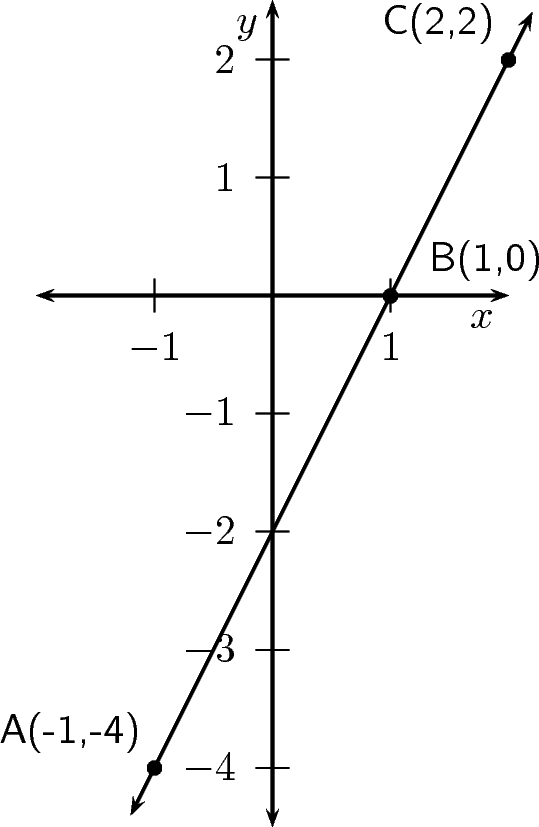
\includegraphics{col11306.imgs/m39213_MG10C12_001.png} % m39213;MG10C12\_001.png;;;6.0;8.5;
      \vspace{2pt}
    \vspace{.1in}
    \end{center}
 \end{figure}       
      \par 
      \label{m39213*id190178}What do you notice about the gradients over each interval?
 \par 
      \label{m39213*id190187}The average gradient of a straight-line function is the same over any two intervals on the function.\par 
    \label{m39213**end}
         \section{ Parabolic and other functions}
    \nopagebreak
            \label{m39223} $ \hspace{-5pt}\begin{array}{cccccccccccc}   
\includegraphics[width=0.75cm]{col11306.imgs/summary_fullmarks.png} &   \end{array} $ \hspace{2 pt}\raisebox{-5 pt}{} {(section shortcode: MG10082 )} \par 
\label{m39223*cid4}
            \subsection{ Average Gradient: Parabolic and other functions}
            \nopagebreak
\label{m39223*secfhsst!!!underscore!!!id252}
            \subsubsection{  Investigation : Average Gradient - Parabolic Function }
            \nopagebreak
      \label{m39223*id190208}Fill in the table by calculating the average gradient over the indicated
intervals for the function $f\left(x\right)=2x-2$:\par 
    % \textbf{m39223*id190240}\par
          \begin{table}[H]
    % \begin{table}[H]
    % \\ '' '0'
        \begin{center}
      \label{m39223*id190240}
    \noindent
    \tabletail{%
        \hline
        \multicolumn{6}{|p{\mytableboxwidth}|}{\raggedleft \small \sl continued on next page}\\
        \hline
      }
      \tablelasttail{}
      \begin{xtabular}[t]{|l|l|l|l|l|l|}\hline
         &
                ${x}_{1}$
               &
                ${x}_{2}$
               &
                ${y}_{1}$
               &
                ${y}_{2}$
               &
                $\frac{{y}_{2}-{y}_{1}}{{x}_{2}-{x}_{1}}$
              % make-rowspan-placeholders
     \tabularnewline\cline{1-1}\cline{2-2}\cline{3-3}\cline{4-4}\cline{5-5}\cline{6-6}
      %--------------------------------------------------------------------
        A-B &
         &
         &
         &
         &
        % make-rowspan-placeholders
     \tabularnewline\cline{1-1}\cline{2-2}\cline{3-3}\cline{4-4}\cline{5-5}\cline{6-6}
      %--------------------------------------------------------------------
        B-C &
         &
         &
         &
         &
        % make-rowspan-placeholders
     \tabularnewline\cline{1-1}\cline{2-2}\cline{3-3}\cline{4-4}\cline{5-5}\cline{6-6}
      %--------------------------------------------------------------------
        C-D &
         &
         &
         &
         &
        % make-rowspan-placeholders
     \tabularnewline\cline{1-1}\cline{2-2}\cline{3-3}\cline{4-4}\cline{5-5}\cline{6-6}
      %--------------------------------------------------------------------
        D-E &
         &
         &
         &
         &
        % make-rowspan-placeholders
     \tabularnewline\cline{1-1}\cline{2-2}\cline{3-3}\cline{4-4}\cline{5-5}\cline{6-6}
      %--------------------------------------------------------------------
        E-F &
         &
         &
         &
         &
        % make-rowspan-placeholders
     \tabularnewline\cline{1-1}\cline{2-2}\cline{3-3}\cline{4-4}\cline{5-5}\cline{6-6}
      %--------------------------------------------------------------------
        F-G &
         &
         &
         &
         &
        % make-rowspan-placeholders
     \tabularnewline\cline{1-1}\cline{2-2}\cline{3-3}\cline{4-4}\cline{5-5}\cline{6-6}
      %--------------------------------------------------------------------
    \end{xtabular}
      \end{center}
    \begin{center}{\small\bfseries Table 10.2}\end{center}
    \begin{caption}{\small\bfseries Table 10.2}\end{caption}
\end{table}
    \par
      \label{m39223*id190636}
What do you notice about the average gradient over each interval? What can you
say about the average gradients between A and D compared to the average
gradients between D and G?\par 
      \label{m39223*id190641}
    \setcounter{subfigure}{0}
	\begin{figure}[H] % horizontal\label{m39223*id190642}
    \begin{center}
    \label{m39223*id190642!!!underscore!!!media}\label{m39223*id190642!!!underscore!!!printimage}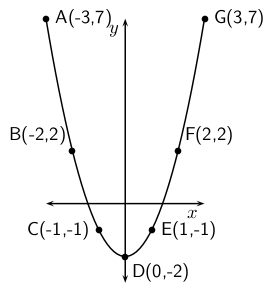
\includegraphics[width=300px]{col11306.imgs/m39223_MG10C12_002.png} % m39223;MG10C12\_002.png;;;6.0;8.5;
      \vspace{2pt}
    \vspace{.1in}
    \end{center}
 \end{figure}       
      \par 
      \label{m39223*id190657}The average gradient of a parabolic function depends on the interval and is the gradient of a straight line that passes through the points on the interval.\par 
      \label{m39223*id190661}For example, in Figure~10.3 the various points have been joined by straight-lines. The average gradients between the joined points are then the gradients of the straight lines that pass through the points.\par 
    \setcounter{subfigure}{0}
	\begin{figure}[H] % horizontal\label{m39223*uid3}
    \begin{center}
    \rule[.1in]{\figurerulewidth}{.005in} \\
        \label{m39223*uid3!!!underscore!!!media}\label{m39223*uid3!!!underscore!!!printimage}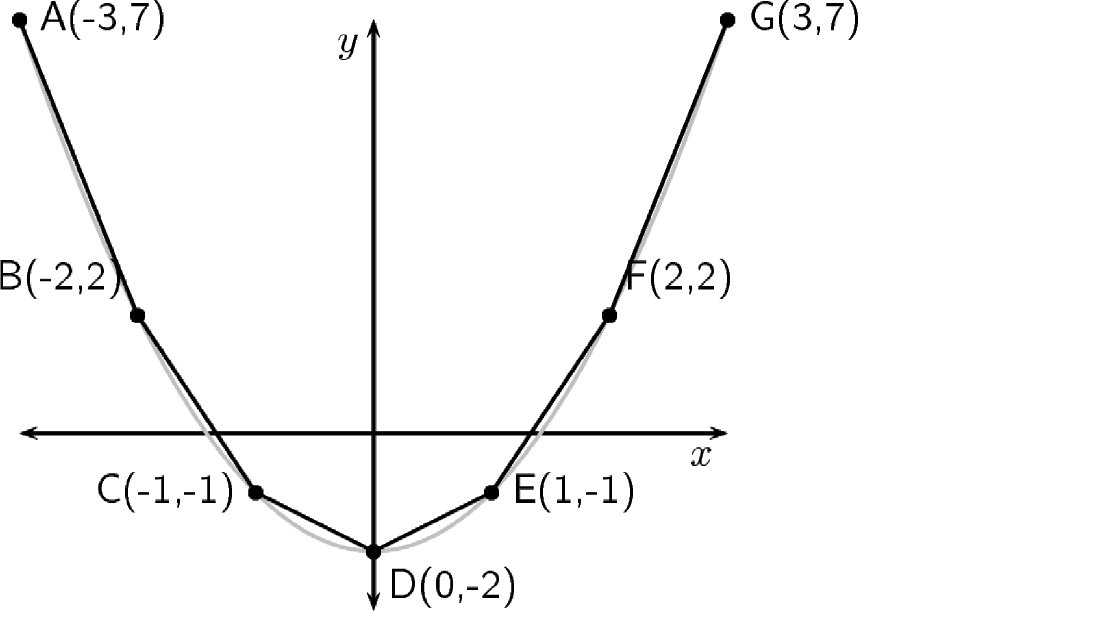
\includegraphics[width=300px]{col11306.imgs/m39223_MG10C12_003.png} % m39223;MG10C12\_003.png;;;6.0;8.5;
      \vspace{2pt}
    \vspace{\rubberspace}\par \begin{cnxcaption}
	  \small \textbf{Figure 10.3: }The average gradient between two points on a curve is the gradient of the straight line that passes through the points.
	\end{cnxcaption}
    \vspace{.1in}
    \rule[.1in]{\figurerulewidth}{.005in} \\
    \end{center}
 \end{figure}       
      \label{m39223*uid4}
            \subsubsection{ Method: Average Gradient}
            \nopagebreak
        \label{m39223*id190691}Given the equation of a curve and two points (${x}_{1}$, ${x}_{2}$):\par 
        \label{m39223*id190722}\begin{enumerate}[noitemsep, label=\textbf{\arabic*}. ] 
            \label{m39223*uid5}\item Write the equation of the curve in the form $y=...$.
\label{m39223*uid6}\item Calculate ${y}_{1}$ by substituting ${x}_{1}$ into the equation for the curve.
\label{m39223*uid7}\item Calculate ${y}_{2}$ by substituting ${x}_{2}$ into the equation for the curve.
\label{m39223*uid8}\item Calculate the average gradient using:
\label{m39223*id189188}\nopagebreak\noindent{}\settowidth{\mymathboxwidth}{\begin{equation}
    \frac{{y}_{2}-{y}_{1}}{{x}_{2}-{x}_{1}}\tag{10.3}
      \end{equation}
    }
    \typeout{Columnwidth = \the\columnwidth}\typeout{math as usual width = \the\mymathboxwidth}
    \ifthenelse{\lengthtest{\mymathboxwidth < \columnwidth}}{% if the math fits, do it again, for real
    \begin{equation}
    \frac{{y}_{2}-{y}_{1}}{{x}_{2}-{x}_{1}}\tag{10.3}
      \end{equation}
    }{% else, if it doesn't fit
    \setlength{\mymathboxwidth}{\columnwidth}
      \addtolength{\mymathboxwidth}{-48pt}
    \par\vspace{12pt}\noindent\begin{minipage}{\columnwidth}
    \parbox[t]{\mymathboxwidth}{\large$
    \frac{{y}_{2}-{y}_{1}}{{x}_{2}-{x}_{1}}$}\hfill
    \parbox[t]{48pt}{\raggedleft 
    (10.3)}
    \end{minipage}\vspace{12pt}\par
    }% end of conditional for this bit of math
    \typeout{math as usual width = \the\mymathboxwidth}
    \end{enumerate}
\par
            \label{m39223*secfhsst!!!underscore!!!id408}\vspace{.5cm} 
      \noindent
      \hspace*{-30pt}
\includegraphics[width=0.5in]{col11306.imgs/pspencil2.png}   \raisebox{25mm}{   
      \begin{mdframed}[linewidth=4, leftmargin=40, rightmargin=40]  
      \begin{exercise}
    \noindent\textbf{Exercise 10.1:  Average Gradient }
        \label{m39223*probfhsst!!!underscore!!!id409}
        \label{m39223*id191077}Find the average gradient of the curve $y=5{x}^{2}-4$ between the points $x=-3$ and $x=3$ \par 
        \vspace{5pt}
        \label{m39223*solfhsst!!!underscore!!!id412}\noindent\textbf{Solution to Exercise } \label{m39223*listfhsst!!!underscore!!!id412}\begin{enumerate}[noitemsep, label=\textbf{Step} \textbf{\arabic*}. ] 
            \leftskip=20pt\rightskip=\leftskip\item  
        \label{m39223*id191151}Label the points as follows:\par 
        \label{m39223*id191154}\nopagebreak\noindent{}
          \settowidth{\mymathboxwidth}{\begin{equation}
    {x}_{1}=-3\tag{10.4}
      \end{equation}
    }
    \typeout{Columnwidth = \the\columnwidth}\typeout{math as usual width = \the\mymathboxwidth}
    \ifthenelse{\lengthtest{\mymathboxwidth < \columnwidth}}{% if the math fits, do it again, for real
    \begin{equation}
    {x}_{1}=-3\tag{10.4}
      \end{equation}
    }{% else, if it doesn't fit
    \setlength{\mymathboxwidth}{\columnwidth}
      \addtolength{\mymathboxwidth}{-48pt}
    \par\vspace{12pt}\noindent\begin{minipage}{\columnwidth}
    \parbox[t]{\mymathboxwidth}{\large$
    {x}_{1}=-3$}\hfill
    \parbox[t]{48pt}{\raggedleft 
    (10.4)}
    \end{minipage}\vspace{12pt}\par
    }% end of conditional for this bit of math
    \typeout{math as usual width = \the\mymathboxwidth}
        \label{m39223*id191178}\nopagebreak\noindent{}
          \settowidth{\mymathboxwidth}{\begin{equation}
    {x}_{2}=3\tag{10.5}
      \end{equation}
    }
    \typeout{Columnwidth = \the\columnwidth}\typeout{math as usual width = \the\mymathboxwidth}
    \ifthenelse{\lengthtest{\mymathboxwidth < \columnwidth}}{% if the math fits, do it again, for real
    \begin{equation}
    {x}_{2}=3\tag{10.5}
      \end{equation}
    }{% else, if it doesn't fit
    \setlength{\mymathboxwidth}{\columnwidth}
      \addtolength{\mymathboxwidth}{-48pt}
    \par\vspace{12pt}\noindent\begin{minipage}{\columnwidth}
    \parbox[t]{\mymathboxwidth}{\large$
    {x}_{2}=3$}\hfill
    \parbox[t]{48pt}{\raggedleft 
    (10.5)}
    \end{minipage}\vspace{12pt}\par
    }% end of conditional for this bit of math
    \typeout{math as usual width = \the\mymathboxwidth}
        \label{m39223*id191200}to make it easier to calculate the gradient.\par 
        \item  
        \label{m39223*id191219}We use the equation for the curve to calculate the $y$-value at ${x}_{1}$ and ${x}_{2}$.\par 
        \label{m39223*id191259}\nopagebreak\noindent{}
          \settowidth{\mymathboxwidth}{\begin{equation}
    \begin{array}{ccc}\hfill {y}_{1}& =& 5x_{1}^{2}-4\hfill \\ & =& 5{\left(-3\right)}^{2}-4\hfill \\ & =& 5\left(9\right)-4\hfill \\ & =& 41\hfill \end{array}\tag{10.6}
      \end{equation}
    }
    \typeout{Columnwidth = \the\columnwidth}\typeout{math as usual width = \the\mymathboxwidth}
    \ifthenelse{\lengthtest{\mymathboxwidth < \columnwidth}}{% if the math fits, do it again, for real
    \begin{equation}
    \begin{array}{ccc}\hfill {y}_{1}& =& 5x_{1}^{2}-4\hfill \\ & =& 5{\left(-3\right)}^{2}-4\hfill \\ & =& 5\left(9\right)-4\hfill \\ & =& 41\hfill \end{array}\tag{10.6}
      \end{equation}
    }{% else, if it doesn't fit
    \setlength{\mymathboxwidth}{\columnwidth}
      \addtolength{\mymathboxwidth}{-48pt}
    \par\vspace{12pt}\noindent\begin{minipage}{\columnwidth}
    \parbox[t]{\mymathboxwidth}{\large$
    {y}_{1}=5x_{1}^{2}-4=5{\left(-3\right)}^{2}-4=5\left(9\right)-4=41$}\hfill
    \parbox[t]{48pt}{\raggedleft 
    (10.6)}
    \end{minipage}\vspace{12pt}\par
    }% end of conditional for this bit of math
    \typeout{math as usual width = \the\mymathboxwidth}
        \label{m39223*id191371}\nopagebreak\noindent{}
          \settowidth{\mymathboxwidth}{\begin{equation}
    \begin{array}{ccc}\hfill {y}_{2}& =& 5x_{2}^{2}-4\hfill \\ & =& 5{\left(3\right)}^{2}-4\hfill \\ & =& 5\left(9\right)-4\hfill \\ & =& 41\hfill \end{array}\tag{10.7}
      \end{equation}
    }
    \typeout{Columnwidth = \the\columnwidth}\typeout{math as usual width = \the\mymathboxwidth}
    \ifthenelse{\lengthtest{\mymathboxwidth < \columnwidth}}{% if the math fits, do it again, for real
    \begin{equation}
    \begin{array}{ccc}\hfill {y}_{2}& =& 5x_{2}^{2}-4\hfill \\ & =& 5{\left(3\right)}^{2}-4\hfill \\ & =& 5\left(9\right)-4\hfill \\ & =& 41\hfill \end{array}\tag{10.7}
      \end{equation}
    }{% else, if it doesn't fit
    \setlength{\mymathboxwidth}{\columnwidth}
      \addtolength{\mymathboxwidth}{-48pt}
    \par\vspace{12pt}\noindent\begin{minipage}{\columnwidth}
    \parbox[t]{\mymathboxwidth}{\large$
    {y}_{2}=5x_{2}^{2}-4=5{\left(3\right)}^{2}-4=5\left(9\right)-4=41$}\hfill
    \parbox[t]{48pt}{\raggedleft 
    (10.7)}
    \end{minipage}\vspace{12pt}\par
    }% end of conditional for this bit of math
    \typeout{math as usual width = \the\mymathboxwidth}
        \item  
        \label{m39223*id191486}\nopagebreak\noindent{}
          \settowidth{\mymathboxwidth}{\begin{equation}
    \begin{array}{ccc}\hfill \frac{{y}_{2}-{y}_{1}}{{x}_{2}-{x}_{1}}& =& \frac{41-41}{3-\left(-3\right)}\hfill \\ & =& \frac{0}{3+3}\hfill \\ & =& \frac{0}{6}\hfill \\ & =& 0\hfill \end{array}\tag{10.8}
      \end{equation}
    }
    \typeout{Columnwidth = \the\columnwidth}\typeout{math as usual width = \the\mymathboxwidth}
    \ifthenelse{\lengthtest{\mymathboxwidth < \columnwidth}}{% if the math fits, do it again, for real
    \begin{equation}
    \begin{array}{ccc}\hfill \frac{{y}_{2}-{y}_{1}}{{x}_{2}-{x}_{1}}& =& \frac{41-41}{3-\left(-3\right)}\hfill \\ & =& \frac{0}{3+3}\hfill \\ & =& \frac{0}{6}\hfill \\ & =& 0\hfill \end{array}\tag{10.8}
      \end{equation}
    }{% else, if it doesn't fit
    \setlength{\mymathboxwidth}{\columnwidth}
      \addtolength{\mymathboxwidth}{-48pt}
    \par\vspace{12pt}\noindent\begin{minipage}{\columnwidth}
    \parbox[t]{\mymathboxwidth}{\large$
    \frac{{y}_{2}-{y}_{1}}{{x}_{2}-{x}_{1}}=\frac{41-41}{3-\left(-3\right)}=\frac{0}{3+3}=\frac{0}{6}=0$}\hfill
    \parbox[t]{48pt}{\raggedleft 
    (10.8)}
    \end{minipage}\vspace{12pt}\par
    }% end of conditional for this bit of math
    \typeout{math as usual width = \the\mymathboxwidth}
        \item  
        \label{m39223*id191621}The average gradient between $x=-3$ and $x=3$ on the curve $y=5{x}^{2}-4$ is 0.
 \par 
        \end{enumerate}
    \end{exercise}
    \end{mdframed}
    }
    \noindent
\label{m39223*secfhsst356}
            \subsection{ Average gradient for other functions}
            \nopagebreak
\label{m39223*id7342}We can extend the concept of average gradient to any function. The average gradient for any function also depends on the interval chosen and is the gradient of a straight line that passes through the two points. So we can use the formula that we found for the average gradient of parabolic functions and apply it to any function. We will consider the average gradient of just two functions here: exponential functions and hyperbolic functions.
\par 
\label{m39223*cid452}
            \subsubsection{ Average gradient of exponential functions}
            \nopagebreak
\label{m39223*id734}For example, if we were asked to find the average gradient of the function $\mathrm{g\left(x\right)}=3.{2}^{x}+2$ between the points $\left(-4;\mathrm{2,2}\right)$ and $\left(-0,6;4\right)$. This is shown in Figure~10.4. 
    \setcounter{subfigure}{0}
	\begin{figure}[H] % horizontal\label{m39223*uid31}
    \begin{center}
    \label{m39223*uid31!!!underscore!!!media}\label{m39223*uid31!!!underscore!!!printimage}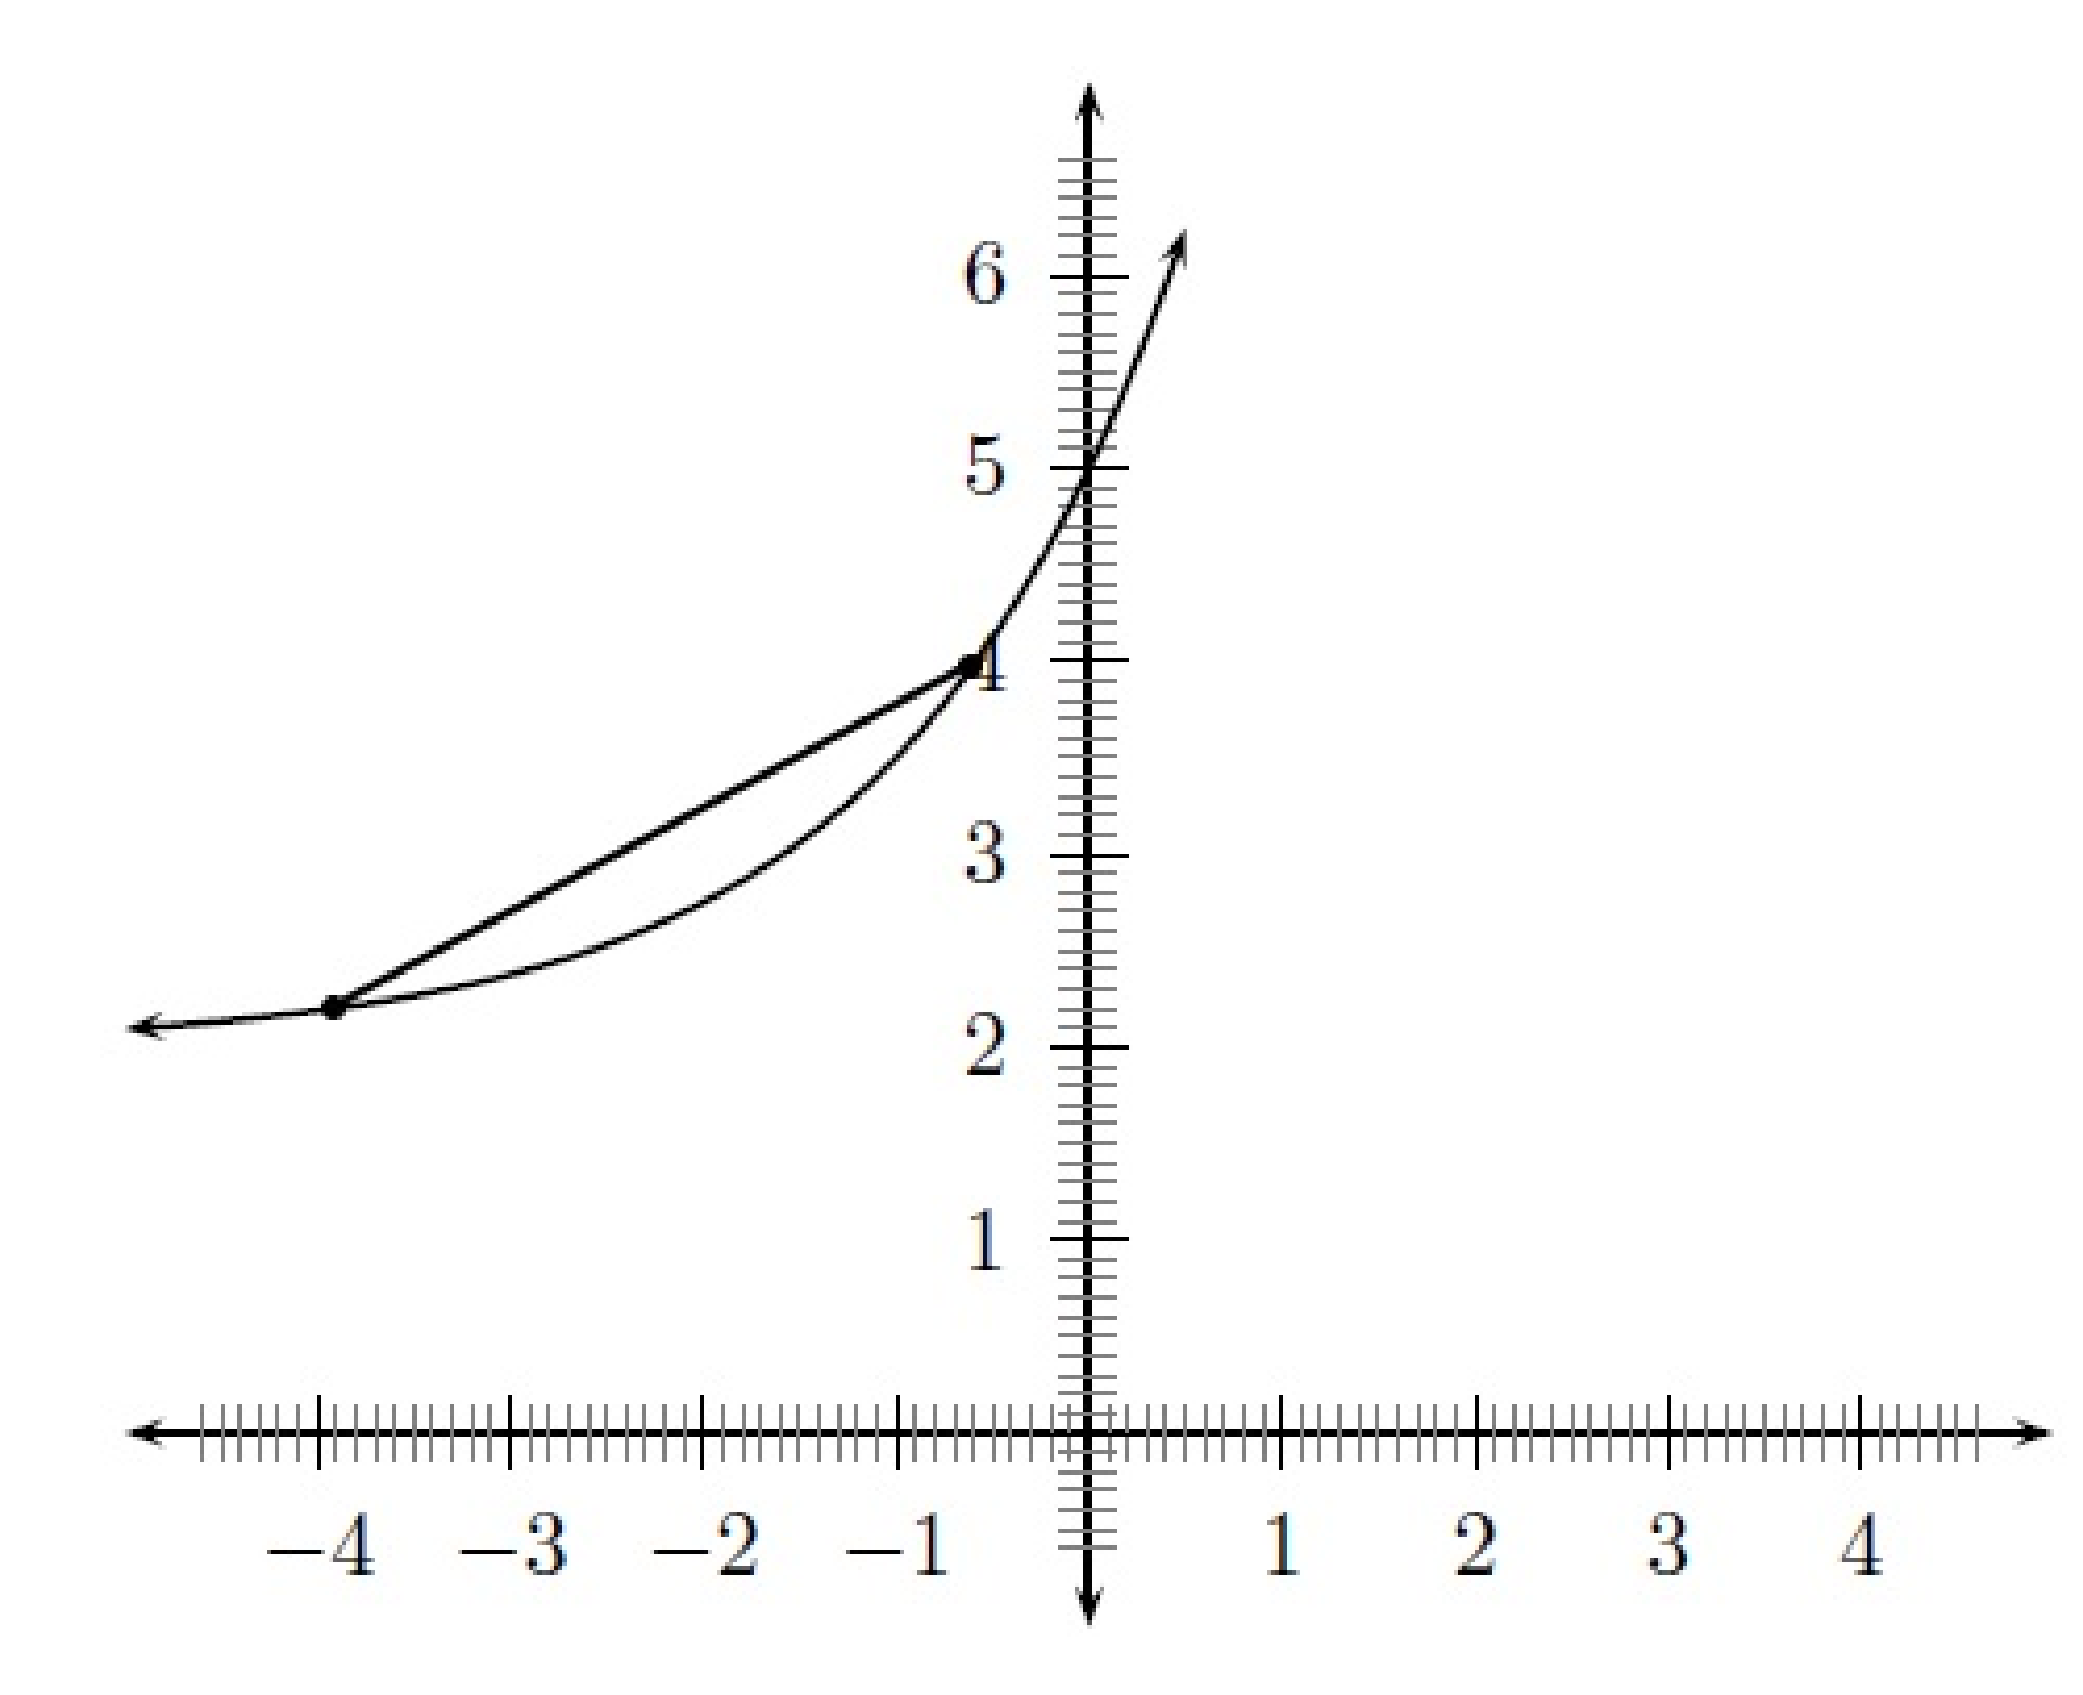
\includegraphics[width=300px]{col11306.imgs/m39223_exponent.png} % m39223;exponent.png;;;6.0;8.5;
      \vspace{2pt}
    \vspace{\rubberspace}\par \begin{cnxcaption}
	  \small \textbf{Figure 10.4: }The average gradient for an exponential function.
	\end{cnxcaption}
    \vspace{.1in}
    \end{center}
 \end{figure}       
Using the formula we find:
 \label{m39223*id193486}\nopagebreak\noindent{}
          \settowidth{\mymathboxwidth}{\begin{equation}
    \begin{array}{ccc}\hfill \frac{{y}_{2}-{y}_{1}}{{x}_{2}-{x}_{1}}& =& \frac{4-2,2}{\left(-0,6\right)-\left(-4\right)}\hfill \\ & =& \frac{1,8}{-0,6+4}\hfill \\ & =& \frac{1,8}{5,2}\hfill \\ & =& 0,35\hfill \end{array}\tag{10.9}
      \end{equation}
    }
    \typeout{Columnwidth = \the\columnwidth}\typeout{math as usual width = \the\mymathboxwidth}
    \ifthenelse{\lengthtest{\mymathboxwidth < \columnwidth}}{% if the math fits, do it again, for real
    \begin{equation}
    \begin{array}{ccc}\hfill \frac{{y}_{2}-{y}_{1}}{{x}_{2}-{x}_{1}}& =& \frac{4-2,2}{\left(-0,6\right)-\left(-4\right)}\hfill \\ & =& \frac{1,8}{-0,6+4}\hfill \\ & =& \frac{1,8}{5,2}\hfill \\ & =& 0,35\hfill \end{array}\tag{10.9}
      \end{equation}
    }{% else, if it doesn't fit
    \setlength{\mymathboxwidth}{\columnwidth}
      \addtolength{\mymathboxwidth}{-48pt}
    \par\vspace{12pt}\noindent\begin{minipage}{\columnwidth}
    \parbox[t]{\mymathboxwidth}{\large$
    \frac{{y}_{2}-{y}_{1}}{{x}_{2}-{x}_{1}}=\frac{4-2,2}{\left(-0,6\right)-\left(-4\right)}=\frac{1,8}{-0,6+4}=\frac{1,8}{5,2}=0,35$}\hfill
    \parbox[t]{48pt}{\raggedleft 
    (10.9)}
    \end{minipage}\vspace{12pt}\par
    }% end of conditional for this bit of math
    \typeout{math as usual width = \the\mymathboxwidth}
\par 
\label{m39223*cid442}
            \subsubsection{ Average gradient of hyperbolic functions}
            \nopagebreak
\label{m39223*id67324}For example, if we were asked to find the average gradient of the function $g\left(x\right)=\frac{2}{x}+2$ between the points $\left(-4;-2,5\right)$ and $\left(0,5;6\right)$ and $\left(-4;2,2\right)$ and $\left(-0,6;4\right)$. This is shown in Figure~10.5.
    \setcounter{subfigure}{0}
	\begin{figure}[H] % horizontal\label{m39223*uid32}
    \begin{center}
    \label{m39223*uid32!!!underscore!!!media}\label{m39223*uid32!!!underscore!!!printimage}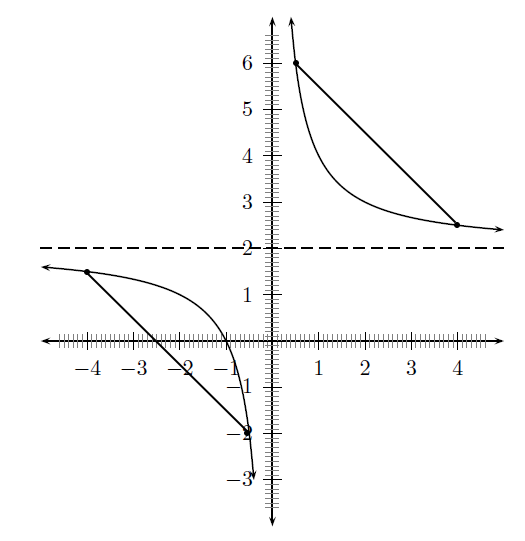
\includegraphics[height=300px]{col11306.imgs/m39223_hyperbola.png} % m39223;hyperbola.png;;;6.0;8.5;
      \vspace{2pt}
    \vspace{\rubberspace}\par \begin{cnxcaption}
	  \small \textbf{Figure 10.5: }The average gradient for a hyperbolic function.
	\end{cnxcaption}
    \vspace{.1in}
    \end{center}
 \end{figure}       \par 
\label{m39223*id2322} For the first point we would get:
 \label{m39223*id196486}\nopagebreak\noindent{}\settowidth{\mymathboxwidth}{\begin{equation}
    \begin{array}{ccc}\hfill \frac{{y}_{2}-{y}_{1}}{{x}_{2}-{x}_{1}}& =& \frac{\left(-2,5\right)-1}{\left(-4\right)-0,5}\hfill \\ & =& \frac{-3,5}{-4,5}\hfill \\ & =& 0,78\hfill \end{array}\tag{10.10}
      \end{equation}
    }
    \typeout{Columnwidth = \the\columnwidth}\typeout{math as usual width = \the\mymathboxwidth}
    \ifthenelse{\lengthtest{\mymathboxwidth < \columnwidth}}{% if the math fits, do it again, for real
    \begin{equation}
    \begin{array}{ccc}\hfill \frac{{y}_{2}-{y}_{1}}{{x}_{2}-{x}_{1}}& =& \frac{\left(-2,5\right)-1}{\left(-4\right)-0,5}\hfill \\ & =& \frac{-3,5}{-4,5}\hfill \\ & =& 0,78\hfill \end{array}\tag{10.10}
      \end{equation}
    }{% else, if it doesn't fit
    \setlength{\mymathboxwidth}{\columnwidth}
      \addtolength{\mymathboxwidth}{-48pt}
    \par\vspace{12pt}\noindent\begin{minipage}{\columnwidth}
    \parbox[t]{\mymathboxwidth}{\large$
    \frac{{y}_{2}-{y}_{1}}{{x}_{2}-{x}_{1}}=\frac{\left(-2,5\right)-1}{\left(-4\right)-0,5}=\frac{-3,5}{-4,5}=0,78$}\hfill
    \parbox[t]{48pt}{\raggedleft 
    (10.10)}
    \end{minipage}\vspace{12pt}\par
    }% end of conditional for this bit of math
    \typeout{math as usual width = \the\mymathboxwidth}
Similarly for the second points we would find that the average gradient is: $0,53$
\par 
\label{m39223**end}
         \section{ Summary and exercises}
    \nopagebreak
            \label{m39240} $ \hspace{-5pt}\begin{array}{cccccccccccc}   \end{array} $ \hspace{2 pt}\raisebox{-5 pt}{
\includegraphics[width=0.5cm]{col11306.imgs/summary_www.png}} {(section shortcode: MG10083 )} \par 
\label{m39240*eip-479}
            \subsection{ Average Gradient: Summary and exercises}
            \nopagebreak
\label{m39240*eip-922}\begin{itemize}[noitemsep]
            \item The average gradient between two points is: $\frac{{y}_{2}-{y}_{1}}{{x}_{2}-{x}_{1}}$\item The average gradient of a straight-line function is the same over any two intervals on the function\item The average gradient of a parabolic function depends on the interval and is the gradient of a straight line that passes through the points on the interval\item We can extend the concept of average gradient to any function\end{itemize}
        \label{m39240*cid5}
            \subsection{ End of Chapter Exercises}
            \nopagebreak
            \label{m39240*id191703}\begin{enumerate}[noitemsep, label=\textbf{\arabic*}. ] 
            \label{m39240*uid9}\item An object moves according to the function $d=2{t}^{2}+1$ , where $d$ is the distance in metres and $t$ the time in seconds. Calculate the average speed of the object between 2 and 3 seconds. The speed is the gradient of the function $d$\newline
\label{m39240*uid10}\item Given: $f\left(x\right)={x}^{3}-6x$.
Determine the average gradient between the points where $x=1$ and $x=4$.\newline
\label{m39240*uid111}\item Find the average gradient of each of the following functions between the points where $x=2$ and $x=3$
\label{m39240*id62342}\begin{enumerate}[noitemsep, label=\textbf{\alph*}. ] 
            \item $f\left(x\right)={x}^{2}+3$\item $f\left(x\right)=\frac{4}{x}+1$\item $f\left(x\right)={2}^{x}-3$\end{enumerate}
\end{enumerate}
  \label{m39240**end}
  \label{3b3f311aa3ebba82678f2a2244617492**end}
\par \raisebox{-5 pt}{
\includegraphics[width=0.5cm]{col11306.imgs/summary_www.png}} Find the answers with the shortcodes:
 \par \begin{tabular}[h]{cccccc}
 (1.) llP  &  (2.) llE  &  (3.) lT5  & \end{tabular}
